

\section*{React}


React es una biblioteca de Javascript para crear interfaces de usuario
lanzada por Facebook en 2013.
Tiene tres características que la definen y distinguen  de otras
biblioteca o frameworks y son:
\begin{itemize}
\item {} 
Es \textbf{declarativa}, ya que permite crear interfaces de manera sencilla. Sólo se diseña una vista para cada estado de la aplicación; React actualizará de manera eficiente y \sphinxstylestrong{rederizará} los componentes correctos cuando los datos cambian.

\item {} 
Está \sphinxstylestrong{basado en componentes}, construye componentes encapsulados que manejan su propio estado, después se integran con otros para hacer IU más complejas.

\item {} 
React puede \sphinxstyleemphasis{renderizar} sobre un servidor usando node o en dispositivos móviles con React Native.

\end{itemize}


Los \textit{componentes} dividen la IU en piezas independientes y reutilizables; además
permite pensar en cada una de manera aislada.
Conceptualmente, los componentes son como funciones de Javascript. Aceptan
entradas arbitrarias llamadas \texttt{props}, abreviación de propiedades, y regresan elementos
de React describiendo lo que debe aparecer en la pantalla.

Los \textit{elementos} son los bloques más básicos en las aplicaciones de React. Un elemento
describe todo que se quiere visualizar en la pantalla.

\fvset{hllines={, ,}}%
\begin{sphinxVerbatim}[commandchars=\\\{\}]
\PYG{n}{const} \PYG{n}{element} \PYG{o}{=} \PYG{o}{\PYGZlt{}}\PYG{n}{h1}\PYG{o}{\PYGZgt{}}\PYG{n}{Hola} \PYG{n}{mundo}\PYG{o}{\PYGZlt{}}\PYG{o}{/}\PYG{n}{h1}\PYG{o}{\PYGZgt{}}
\end{sphinxVerbatim}


El método \texttt{render} regresa una descripción
de que es lo que se quiere ver en la pantalla. React
toma esa descripción y muestra el resultado. En
particular, \texttt{render} retorna un elemento de React,
que es una descripción ligera de lo que se quiere 
renderizar.

Para el desarrollo de una aplicación en React se utiliza
una sintaxis especial llamada \textit{JSX} (JavaScript XML), que no
es requerida, pero al ser una extensión de JavaScript que permite
utilizar un código parecido al HTML con todo el poder de JavaScript
se cumple el objetivo de React de no separar la lógica de renderizado
y la de la interfaz de usuario.


\subsection*{Ejemplo de una aplicación}

La manera más simple para crear una aplicación en
React es a través del kit inicial sin
configuraciones para React lanzado por Facebook
llamado \texttt{create-react-app}.

Para iniciar con esta herramienta primero se instala a través del
manejador de paquetes de node, \texttt{npm}:

\fvset{hllines={, ,}}%
\begin{sphinxVerbatim}[commandchars=\\\{\}]
npm install \PYGZhy{}g create\PYGZhy{}react\PYGZhy{}app
\end{sphinxVerbatim}


Ahora se puede crear y lanzar una aplicación con React. 

\fvset{hllines={, ,}}%
\begin{sphinxVerbatim}[commandchars=\\\{\}]
create\PYGZhy{}react\PYGZhy{}app ejemplo\PYGZus{}react\PYGZus{}app
\PYG{n+nb}{cd} react\PYGZus{}ejemplo\PYGZus{}app
\end{sphinxVerbatim}

La estructura del directorio creado es la siguiente:

\fvset{hllines={, ,}}%
\begin{sphinxVerbatim}[commandchars=\\\{\}]
ejemplo\PYGZus{}react\PYGZus{}app/
├── node\PYGZus{}modules
├── package.json
├── package\PYGZhy{}lock.json
├── public
│   ├── favicon.ico
│   ├── index.html
│   └── manifest.json
├── README.md
└── src
    ├── App.css
    ├── App.js
    ├── App.test.js
    ├── index.css
    ├── index.js
    ├── logo.svg
    └── registerServiceWorker.js
\end{sphinxVerbatim}

\begin{itemize}
\item {} 
\sphinxstylestrong{node\_modules/}. Contiene todos los paquetes de node que fueron instalados vía npm. Como se usó create-react-app, algunos módulos ya fueron instalados.

\item {} 
\sphinxstylestrong{package.json}. El archivo que muestra las lista de dependencias y otras opciones de configuración del proyecto.

\item {} 
\sphinxstylestrong{.gitignore}. Este archivo indica todos los archivos y carpetas que nos deben añadirse a un repositorio remoto cuando se usa git.

\item {} 
\sphinxstylestrong{public/}. Esta carpeta guarda todos los archivos cuando se despliega un proyecto en modo de producción.

\end{itemize}

En un principio todo lo que se necesita está localizado en la carpeta \sphinxstyleemphasis{src/}.
El enfoque principal está dirigido al archivo \sphinxstyleemphasis{src/App.js} para implementar los
componentes de React. Este se usa para implementar la aplicación, pero con el
crecimiento de un proyecto siempre es necesario dividir los componentes en
múltiples archivos, donde cada archivo mantiene uno o algunos componentes por
su cuenta.

La aplicación generada con \sphinxstyleemphasis{create-react-app} es un proyecto de npm. Se puede usar
npm para instalar o eliminar paquetes de node. Además viene con los siguientes
scripts de npm para la línea de comandos.

\fvset{hllines={, ,}}%
\begin{sphinxVerbatim}[commandchars=\\\{\}]
\PYG{c+c1}{\PYGZsh{} Ejecuta la aplicación en http://localhost:3000}
npm start

\PYG{c+c1}{\PYGZsh{} Ejecutar los tests}
npm \PYG{n+nb}{test}

\PYG{c+c1}{\PYGZsh{} Construye la aplicación para producción}
npm run build
\end{sphinxVerbatim}

Esos scripts están definidos en el \sphinxstyleemphasis{package.json}.

El siguiente fragmento de código muestra una subclase
de \texttt{React.Component} llamada \texttt{PodcastsList}.


\fvset{hllines={, ,}}%
\begin{sphinxVerbatim}[commandchars=\\\{\}]
class PodcastsList extends React.Component \PYGZob{}
  render() \PYGZob{}
    return (
      \PYG{p}{\PYGZlt{}}\PYG{n+nt}{div} \PYG{n+na}{className}\PYG{o}{=}\PYG{l+s}{\PYGZdq{}podcast\PYGZhy{}list\PYGZdq{}}\PYG{p}{\PYGZgt{}}
        \PYG{p}{\PYGZlt{}}\PYG{n+nt}{h1}\PYG{p}{\PYGZgt{}}Podcasts for \PYGZob{}this.props.name\PYGZcb{}\PYG{p}{\PYGZlt{}}\PYG{p}{/}\PYG{n+nt}{h1}\PYG{p}{\PYGZgt{}}
        \PYG{p}{\PYGZlt{}}\PYG{n+nt}{ul}\PYG{p}{\PYGZgt{}}
          \PYG{p}{\PYGZlt{}}\PYG{n+nt}{li}\PYG{p}{\PYGZgt{}}Simulacro\PYG{p}{\PYGZlt{}}\PYG{p}{/}\PYG{n+nt}{li}\PYG{p}{\PYGZgt{}}
          \PYG{p}{\PYGZlt{}}\PYG{n+nt}{li}\PYG{p}{\PYGZgt{}}Olallo Rubio\PYG{p}{\PYGZlt{}}\PYG{p}{/}\PYG{n+nt}{li}\PYG{p}{\PYGZgt{}}
          \PYG{p}{\PYGZlt{}}\PYG{n+nt}{li}\PYG{p}{\PYGZgt{}}Revolver\PYG{p}{\PYGZlt{}}\PYG{p}{/}\PYG{n+nt}{li}\PYG{p}{\PYGZgt{}}
        \PYG{p}{\PYGZlt{}}\PYG{p}{/}\PYG{n+nt}{ul}\PYG{p}{\PYGZgt{}}
      \PYG{p}{\PYGZlt{}}\PYG{p}{/}\PYG{n+nt}{div}\PYG{p}{\PYGZgt{}}
    );
  \PYGZcb{}
\PYGZcb{}
\end{sphinxVerbatim}

Una forma de añadir la clase anterior a nuestro proyecto
en \sphinxcode{\sphinxupquote{create-react-app}} es modificando el archivo \sphinxcode{\sphinxupquote{index.js}} dentro
de \sphinxstyleemphasis{src/} cambiando \sphinxcode{\sphinxupquote{\textless{}App \textgreater{}}} por el \sphinxcode{\sphinxupquote{\textless{} PodcastsList name="Donkey" /\textgreater{}}}, si la aplicación
se está ejecutando solo se mostrará el mensaje y ningún otro elemento de los
generados por \sphinxcode{\sphinxupquote{create-react-app}}.


\begin{figure}[ht]
\centering
\caption{Resultado de la aplicación en un navegador.}
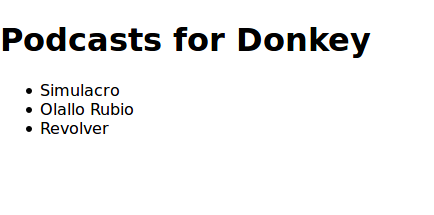
\includegraphics[scale=0.3]{react_first_app}
\end{figure}


\section*{Anexo IX: Firebase para aplicaciones web}

Para utilizar los servicios Firebase en una aplicación web
se siguen los mismos pasos que para el caso de 
aplicaciones para Android. Desde la consola de Firebase
se crea el proyecto y se obtiene un fragmento de código
de inicialización. Ese código  contiene información de inicialización para configurar el SDK de Firebase JavaScript a fin de usar Authentication, Cloud Storage, Realtime Database y Cloud Firestore.


Se puede acceder
a cada servicio desde el espacio de nombres de \sphinxcode{\sphinxupquote{firebase}}:
\begin{itemize}
\item {} 
\sphinxcode{\sphinxupquote{firebase.auth()}} - Authentication

\item {} 
\sphinxcode{\sphinxupquote{firebase.storage()}} - Cloud Storage

\item {} 
\sphinxcode{\sphinxupquote{firebase.database()}} - Realtime Database

\item {} 
\sphinxcode{\sphinxupquote{firebase.firestore()}} - Cloud Firestore

\end{itemize}

El proceso para usar el servicio de Realtime Database y Authentication
es el mismo que en Android. Los métodos de lectura y escritura
se mantienen cambiando únicamente la sintaxis.


\subsection*{Firebase Realtime Database}
\label{\detokenize{firebase_web:firebase-realtime-database}}

Para leer la base de datos o escribir en ella, se necesita una instancia de
\sphinxcode{\sphinxupquote{firebase.database.Reference}}:

\fvset{hllines={, ,}}%
\begin{sphinxVerbatim}[commandchars=\\\{\}]
\PYG{o}{/}\PYG{o}{/} \PYG{n}{Obtiene} \PYG{n}{una} \PYG{n}{referencia} \PYG{n}{al} \PYG{n}{servicio} \PYG{n}{de} \PYG{n}{la} \PYG{n}{base} \PYG{n}{de} \PYG{n}{datos}
\PYG{n}{var} \PYG{n}{database} \PYG{o}{=} \PYG{n}{firebase}\PYG{o}{.}\PYG{n}{database}\PYG{p}{(}\PYG{p}{)}\PYG{p}{;}
\end{sphinxVerbatim}


\subsubsection*{Lectura y escritura de datos}
\label{\detokenize{firebase_web:lectura-y-escritura-de-datos}}
Para recuperar los datos de Firebase, se debe agregar un escuchador
asíncrono a \sphinxcode{\sphinxupquote{firebase.database.Reference}}. El escuchador se activa una vez para
el estado inicial de los datos y otra vez cuando los datos cambian.


Para ejecutar operaciones de escritura básicas, puedes usar \sphinxcode{\sphinxupquote{set()}} para guardar
datos en una referencia que especifiques y reemplazar los datos existentes en
esa ruta de acceso. Por ejemplo si se desea añadir un usuario a la base de datos,
una opción es la siguiente:

\fvset{hllines={, ,}}%
\begin{sphinxVerbatim}[commandchars=\\\{\}]
\PYG{n}{function} \PYG{n}{writeUserData}\PYG{p}{(}\PYG{n}{userId}\PYG{p}{,} \PYG{n}{name}\PYG{p}{,} \PYG{n}{email}\PYG{p}{,} \PYG{n}{imageUrl}\PYG{p}{)} \PYG{p}{\PYGZob{}}
\PYG{n}{firebase}\PYG{o}{.}\PYG{n}{database}\PYG{p}{(}\PYG{p}{)}\PYG{o}{.}\PYG{n}{ref}\PYG{p}{(}\PYG{l+s+s1}{\PYGZsq{}}\PYG{l+s+s1}{users/}\PYG{l+s+s1}{\PYGZsq{}} \PYG{o}{+} \PYG{n}{userId}\PYG{p}{)}\PYG{o}{.}\PYG{n}{set}\PYG{p}{(}\PYG{p}{\PYGZob{}}
    \PYG{n}{username}\PYG{p}{:} \PYG{n}{name}\PYG{p}{,}
    \PYG{n}{email}\PYG{p}{:} \PYG{n}{email}\PYG{p}{,}
    \PYG{n}{profile\PYGZus{}picture} \PYG{p}{:} \PYG{n}{imageUrl}
  \PYG{p}{\PYGZcb{}}\PYG{p}{)}\PYG{p}{;}
\PYG{p}{\PYGZcb{}}
\end{sphinxVerbatim}

\sphinxcode{\sphinxupquote{set()}} sobrescribe los datos en la ubicación que se especifica, incluidos
los nodos secundarios.


\subsubsection*{Detección de eventos en valores}
\label{\detokenize{firebase_web:detecta-eventos-en-valores}}
Si deseas leer datos de una ruta de acceso y escuchar para detectar cambios,
usa los métodos \sphinxcode{\sphinxupquote{on()}} o \sphinxcode{\sphinxupquote{once()}} de \sphinxcode{\sphinxupquote{firebase.database.Reference}}
para observar eventos.

El evento más común es \sphinxcode{\sphinxupquote{value}} y permite leer una instantánea estática del
contenido de una ruta de acceso determinada, en el estado en que se encontraba
en el momento del evento. Este método se activa cuando se vincula el escuchador
y se vuelve a activar cada vez que cambian los datos (incluidos los de
nivel secundario). La devolución de llamada del evento recibe una instantánea
que contiene todos los datos de dicha ubicación, incluidos los datos
secundarios. Si no hay datos, la instantánea tiene un valor nulo.

En el siguiente ejemplo se muestra una aplicación donde se recupera el valor
de un recurso en la base de datos:

\fvset{hllines={, ,}}%
\begin{sphinxVerbatim}[commandchars=\\\{\}]
\PYG{n}{var} \PYG{n}{resourceRef} \PYG{o}{=} \PYG{n}{firebase}\PYG{o}{.}\PYG{n}{database}\PYG{p}{(}\PYG{p}{)}\PYG{o}{.}\PYG{n}{ref}\PYG{p}{(}\PYG{l+s+s1}{\PYGZsq{}}\PYG{l+s+s1}{resource}\PYG{l+s+s1}{\PYGZsq{}}\PYG{p}{)}\PYG{p}{;}
\PYG{n}{resourceRef}\PYG{o}{.}\PYG{n}{on}\PYG{p}{(}\PYG{l+s+s1}{\PYGZsq{}}\PYG{l+s+s1}{value}\PYG{l+s+s1}{\PYGZsq{}}\PYG{p}{,} \PYG{n}{function}\PYG{p}{(}\PYG{n}{snapshot}\PYG{p}{)} \PYG{p}{\PYGZob{}}
  \PYG{n}{showValueOnScreen}\PYG{p}{(}\PYG{n}{snapshot}\PYG{o}{.}\PYG{n}{val}\PYG{p}{(}\PYG{p}{)}\PYG{p}{)}\PYG{p}{;}
\PYG{p}{\PYGZcb{}}\PYG{p}{)}\PYG{p}{;}
\end{sphinxVerbatim}

El escuchador recibe una \sphinxcode{\sphinxupquote{snapshot}} que contiene los datos de la ubicación
especifica en la base de datos en el momento del evento. Se pueden recuperar
los datos de la \sphinxcode{\sphinxupquote{snapshot}} con el método \sphinxcode{\sphinxupquote{val()}}.


\subsubsection*{Actualizar o borrar datos}
\label{\detokenize{firebase_web:actualizar-o-borrar-datos}}
Para escribir de forma simultánea en elementos secundarios específicos de un
nodo sin sobrescribir otros nodos secundarios, usa el método \sphinxcode{\sphinxupquote{update()}}.

También existe el método \sphinxcode{\sphinxupquote{push()}} para añadir una entrada con un identificador
único sobre una referencia.

La forma más sencilla de borrar datos es llamar a \sphinxcode{\sphinxupquote{remove()}} en una referencia a
la ubicación de los datos. Para borrar, también puedes especificar nulo como
el valor de otra operación de escritura, como \sphinxcode{\sphinxupquote{set()}} o \sphinxcode{\sphinxupquote{update()}}.


\subsection*{Firebase Authentication}

De este servicio se utilizó la autenticación con
correo electrónico y contraseña.
El SDK de Firebase Authentication proporciona métodos para crear y administrar usuarios que utilizan sus direcciones de correo electrónico y sus contraseñas para acceder.

Para crear una cuenta de usuario nueva se pasa la dirección de correo electrónico y la contraseña del nuevo usuario a \texttt{createUserWithEmailAndPassword} para crear la cuenta nueva.

\fvset{hllines={, ,}}%
\begin{sphinxVerbatim}[commandchars=\\\{\}]
\PYG{n}{firebase}\PYG{o}{.}\PYG{n}{auth}\PYG{p}{(}\PYG{p}{)}\PYG{o}{.}\PYG{n}{createUserWithEmailAndPassword}\PYG{p}{(}\PYG{n}{email}\PYG{p}{,} \PYG{n}{password}\PYG{p}{)}\PYG{o}{.}\PYG{n}{catch}\PYG{p}{(}\PYG{n}{function}\PYG{p}{(}\PYG{n}{error}\PYG{p}{)} \PYG{p}{\PYGZob{}}
  \PYG{o}{/}\PYG{o}{/} \PYG{n}{El} \PYG{n}{manejo} \PYG{n}{de} \PYG{n}{errores} \PYG{n}{va} \PYG{n}{aquí}
  \PYG{n}{var} \PYG{n}{errorCode} \PYG{o}{=} \PYG{n}{error}\PYG{o}{.}\PYG{n}{code}\PYG{p}{;}
  \PYG{n}{var} \PYG{n}{errorMessage} \PYG{o}{=} \PYG{n}{error}\PYG{o}{.}\PYG{n}{message}\PYG{p}{;}
\PYG{p}{\PYGZcb{}}\PYG{p}{)}\PYG{p}{;}
\end{sphinxVerbatim}


Cuando un usuario accede a tus apps, se pasan la dirección de correo electrónico y la contraseña al método \texttt{signInWithEmailAndPassword}.

\fvset{hllines={, ,}}%
\begin{sphinxVerbatim}[commandchars=\\\{\}]
\PYG{n}{firebase}\PYG{o}{.}\PYG{n}{auth}\PYG{p}{(}\PYG{p}{)}\PYG{o}{.}\PYG{n}{signInWithEmailAndPassword}\PYG{p}{(}\PYG{n}{email}\PYG{p}{,} \PYG{n}{password}\PYG{p}{)}\PYG{o}{.}\PYG{n}{catch}\PYG{p}{(}\PYG{n}{function}\PYG{p}{(}\PYG{n}{error}\PYG{p}{)} \PYG{p}{\PYGZob{}}
\PYG{o}{/}\PYG{o}{/} \PYG{n}{Aquí} \PYG{n}{se} \PYG{n}{manejan} \PYG{n}{los} \PYG{n}{errores}
\PYG{n}{var} \PYG{n}{errorCode} \PYG{o}{=} \PYG{n}{error}\PYG{o}{.}\PYG{n}{code}\PYG{p}{;}
\PYG{n}{var} \PYG{n}{errorMessage} \PYG{o}{=} \PYG{n}{error}\PYG{o}{.}\PYG{n}{message}\PYG{p}{;}
\PYG{o}{/}\PYG{o}{/} \PYG{o}{.}\PYG{o}{.}\PYG{o}{.}
\PYG{p}{\PYGZcb{}}\PYG{p}{)}\PYG{p}{;}
\end{sphinxVerbatim}

La manera recomendada de obtener el usuario actual es establecer un observador en el objeto \sphinxcode{\sphinxupquote{Auth}}:

\fvset{hllines={, ,}}%
\begin{sphinxVerbatim}[commandchars=\\\{\}]
\PYG{n}{firebase}\PYG{o}{.}\PYG{n}{auth}\PYG{p}{(}\PYG{p}{)}\PYG{o}{.}\PYG{n}{onAuthStateChanged}\PYG{p}{(}\PYG{n}{function}\PYG{p}{(}\PYG{n}{user}\PYG{p}{)} \PYG{p}{\PYGZob{}}
\PYG{k}{if} \PYG{p}{(}\PYG{n}{user}\PYG{p}{)} \PYG{p}{\PYGZob{}}
  \PYG{o}{/}\PYG{o}{/} \PYG{n}{El} \PYG{n}{usuario} \PYG{n}{ha} \PYG{n}{iniciado} \PYG{n}{sesión}
\PYG{p}{\PYGZcb{}} \PYG{k}{else} \PYG{p}{\PYGZob{}}
  \PYG{o}{/}\PYG{o}{/} \PYG{n}{No} \PYG{n}{hay} \PYG{n}{un} \PYG{n}{usuario} \PYG{n}{activo}
\PYG{p}{\PYGZcb{}}
\PYG{p}{\PYGZcb{}}\PYG{p}{)}\PYG{p}{;}
\end{sphinxVerbatim}

También se puede usar la propiedad \sphinxcode{\sphinxupquote{currentUser}} para obtener el usuario que
accedió. Si un usuario no accedió a su cuenta, \sphinxcode{\sphinxupquote{currentUser}} mostrará un
resultado nulo:

\fvset{hllines={, ,}}%
\begin{sphinxVerbatim}[commandchars=\\\{\}]
\PYG{n}{var} \PYG{n}{user} \PYG{o}{=} \PYG{n}{firebase}\PYG{o}{.}\PYG{n}{auth}\PYG{p}{(}\PYG{p}{)}\PYG{o}{.}\PYG{n}{currentUser}\PYG{p}{;}
\PYG{k}{if} \PYG{p}{(}\PYG{n}{user}\PYG{p}{)} \PYG{p}{\PYGZob{}}
  \PYG{o}{/}\PYG{o}{/} \PYG{n}{El} \PYG{n}{usuario} \PYG{n}{ha} \PYG{n}{iniciado} \PYG{n}{sesión}
\PYG{p}{\PYGZcb{}} \PYG{k}{else} \PYG{p}{\PYGZob{}}
  \PYG{o}{/}\PYG{o}{/} \PYG{n}{No} \PYG{n}{hay} \PYG{n}{un} \PYG{n}{usuario} \PYG{n}{activo}
\PYG{p}{\PYGZcb{}}
\end{sphinxVerbatim}


Para obtener la información del perfil de un usuario, puedes usar las propiedades de una instancia de \texttt{User}. Por ejemplo:

\fvset{hllines={, ,}}%
\begin{sphinxVerbatim}[commandchars=\\\{\}]
\PYG{n}{var} \PYG{n}{user} \PYG{o}{=} \PYG{n}{firebase}\PYG{o}{.}\PYG{n}{auth}\PYG{p}{(}\PYG{p}{)}\PYG{o}{.}\PYG{n}{currentUser}\PYG{p}{;}
\PYG{n}{var} \PYG{n}{name}\PYG{p}{,} \PYG{n}{email}\PYG{p}{,} \PYG{n}{photoUrl}\PYG{p}{,} \PYG{n}{uid}\PYG{p}{,} \PYG{n}{emailVerified}\PYG{p}{;}

\PYG{k}{if} \PYG{p}{(}\PYG{n}{user} \PYG{o}{!=} \PYG{n}{null}\PYG{p}{)} \PYG{p}{\PYGZob{}}
  \PYG{n}{name} \PYG{o}{=} \PYG{n}{user}\PYG{o}{.}\PYG{n}{displayName}\PYG{p}{;}
  \PYG{n}{email} \PYG{o}{=} \PYG{n}{user}\PYG{o}{.}\PYG{n}{email}\PYG{p}{;}
  \PYG{n}{photoUrl} \PYG{o}{=} \PYG{n}{user}\PYG{o}{.}\PYG{n}{photoURL}\PYG{p}{;}
  \PYG{n}{emailVerified} \PYG{o}{=} \PYG{n}{user}\PYG{o}{.}\PYG{n}{emailVerified}\PYG{p}{;}
  \PYG{n}{uid} \PYG{o}{=} \PYG{n}{user}\PYG{o}{.}\PYG{n}{uid}\PYG{p}{;}  \PYG{o}{/}\PYG{o}{/} \PYG{n}{El} \PYG{n+nb}{id} \PYG{k}{del} \PYG{n}{usuario} \PYG{n}{es} \PYG{n}{único} \PYG{n}{en} \PYG{n}{un} \PYG{n}{proyecto} \PYG{n}{de} \PYG{n}{Firebase}

\PYG{p}{\PYGZcb{}}
\end{sphinxVerbatim}


Para salir de la sesión de un usuario, se llama a \sphinxcode{\sphinxupquote{signOut}}:

\fvset{hllines={, ,}}%
\begin{sphinxVerbatim}[commandchars=\\\{\}]
\PYG{n}{firebase}\PYG{o}{.}\PYG{n}{auth}\PYG{p}{(}\PYG{p}{)}\PYG{o}{.}\PYG{n}{signOut}\PYG{p}{(}\PYG{p}{)}\PYG{o}{.}\PYG{n}{then}\PYG{p}{(}\PYG{n}{function}\PYG{p}{(}\PYG{p}{)} \PYG{p}{\PYGZob{}}
\PYG{o}{/}\PYG{o}{/} \PYG{n}{Se} \PYG{n}{cierra} \PYG{n}{la} \PYG{n}{sesión} \PYG{n}{exitosamente}
\PYG{p}{\PYGZcb{}}\PYG{p}{)}\PYG{o}{.}\PYG{n}{catch}\PYG{p}{(}\PYG{n}{function}\PYG{p}{(}\PYG{n}{error}\PYG{p}{)} \PYG{p}{\PYGZob{}}
  \PYG{o}{/}\PYG{o}{/} \PYG{n}{Un} \PYG{n}{error} \PYG{n}{ocurrió}
\PYG{p}{\PYGZcb{}}\PYG{p}{)}\PYG{p}{;}
\end{sphinxVerbatim}


\subsection*{Firebase Hosting}
\label{\detokenize{firebase_web:firebase-hosting}}

Este servicio permite implementar y alojar los recursos estáticos de una aplicación
fácilmente (HTML, CSS, JavaScript, etc.). Todo el contenido se transmite a través
de HTTPS y está respaldado por una CDN global.

La ruta de implementación es la siguiente:

\begin{itemize}

\item{Instalar Firebase CLI.}
\label{\detokenize{firebase_web:instalar-firebase-cli}}
La CLI (interfaz de línea de comandos) de Firebase necesita Node.js y npm.

Para instalar Firebase CLI a través de npm se escribe los siguiente:

\fvset{hllines={, ,}}%
\begin{sphinxVerbatim}[commandchars=\\\{\}]
\PYG{n}{npm} \PYG{n}{install} \PYG{o}{\PYGZhy{}}\PYG{n}{g} \PYG{n}{firebase}\PYG{o}{\PYGZhy{}}\PYG{n}{tools}
\end{sphinxVerbatim}

Esto instala el comando \sphinxcode{\sphinxupquote{firebase}} de manera global.


\item\textbf{Inicializar la aplicación.}
\label{\detokenize{firebase_web:inicializar-la-aplicacion}}
Si se ejecuta el comando \sphinxcode{\sphinxupquote{firebase init}}, se crea un archivo de configuración
\sphinxcode{\sphinxupquote{firebase.json}} en la raíz del directorio del proyecto.


\item\textbf{Agregar un archivo.}
\label{\detokenize{firebase_web:agregar-un-archivo}}
Cuando se inicializa una aplicación, se pedirá proporcionar un directorio para
usarlo como raíz pública (el valor predeterminado es «public»). Si aún no
se tiene un archivo index.html válido en tu directorio raíz público, se creará
uno.


\item\textbf{Lanzar un sitio web.}
\label{\detokenize{firebase_web:implementar-un-sitio-web}}
Ejecutar \sphinxcode{\sphinxupquote{firebase deploy}} implementará la aplicación en el dominio
\sphinxcode{\sphinxupquote{\textless{}APP-DE-FIREBASE\textgreater{}.firebaseapp.com}}

\end{itemize}